\newcommand{\docNome}{Piano di Qualifica}                          % NOME DEL DOCUMENTO
\newcommand{\docVersione}{2.0.0}                 % INSERIRE VERSIONE IN FORMATO x.y.z
\newcommand{\docStatus}{in lavorazione}          % AGGIORNARE SOLO QUANDO APPROVATO
\newcommand{\docUso}{Esterno}                           % INTERNO O ESTERNO
\newcommand{\docDestinatari}{
      Gruppo Sweven Team\\ %aggiungere altri con & Nome\\
      & Prof. Tullio Vardanega\\
      & Prof. Riccardo Cardin\\
      & Azienda Imola Informatica\\
} 
\newcommand{\docNomeTeam}{Sweven Team}
\newcommand{\docRedattori}{
	Pietro Macrì\\
	& Mattia Episcopo\\
      & Samuele Rizzato\\
      & Irene Benetazzo\\
}
\newcommand{\docVerificatori}{
      Tommaso Berlaffa\\
      & Pietro Macrì\\
      & Irene Benetazzo\\
}
\newcommand{\docApprovazione}{Qi Fan Andrea Pan}
\newcommand{\glossario}[1]{\textit{#1}\textsubscript{\textit{G}}}
\documentclass[12pt, a4paper,table]{article}
\usepackage[T1]{fontenc}
\usepackage[utf8]{inputenc}
\usepackage{lastpage}
\usepackage{fancyhdr}
\usepackage{fancyvrb}
\usepackage{geometry}
\usepackage{xcolor}
\usepackage{array}
\usepackage{graphicx}
\usepackage{float}
\usepackage{charter}
\usepackage{eurosym}
\usepackage{pdflscape}
\usepackage{longtable}
\usepackage{hyperref}
\hypersetup{
pdfborder = {0 0 0}
}
\geometry{a4paper,top=3cm,bottom=3cm,left=2cm,right=2cm}
\title{\textsc{\docNome}}
\author{}
\date{}
\definecolor{footer-gray}{HTML}{808080}
\pagestyle{fancy}
\fancyhf{}
\rhead{\textcolor{footer-gray}{\docNome} }
\lhead{\textcolor{footer-gray}{Sweven Team}}
\fancyfoot{}
\cfoot{\textcolor{footer-gray}{Pagina \thepage  \hspace{1pt} di \pageref*{LastPage}} }
\setcounter{tocdepth}{5}	%aggiunge paragrafi e sottoparagrafi all'indice
\setcounter{secnumdepth}{5}	%aggiunge numero indicizazzione a paragrafi e sottoparagrafi
\renewcommand*\contentsname{Indice}
\begin{document}
\maketitle
	\vspace{-3em}
	\begin{center}
	
\includegraphics[scale=0.50]{images/logo.jpg} \\
	\vspace{2em}
	\huge \textsc{\docNomeTeam}\\
	\normalsize \href{mailto:swe7.team@gmail.com}{swe7.team@gmail.com}\\
	\vspace{2em}
	\begin{tabular}{r|l}
		\multicolumn{2}{c}{ \textsc{Informazioni sul documento} } \\
		\hline
		\textbf{Versione}     & \docVersione\\
		\textbf{Uso}          & \docUso\\
        \textbf{Destinatari}  & \docDestinatari\\
		\textbf{Stato}        & \docStatus\\
		\textbf{Redattori}    & \docRedattori\\
		\textbf{Verificatori} & \docVerificatori\\
		\textbf{Approvatori} & \docApprovazione\\
	\end{tabular}
	\end{center}
    \vspace{3em}
    \begin{center}
        \LARGE{\textbf{Sintesi}} 
    \end{center}
    \normalsize{Guida per l'utente del prodotto \glossario{Chatbot}.}
	\thispagestyle{empty}   
	\newpage
\section*{Diario delle modifiche}
	\begin{center}
	\renewcommand{\arraystretch}{1.8} %aumento ampiezza righe
	\begin{longtable}{ |c|c|p{8em}|c|m{5em}|m{6em}| }
	\hline
	\textbf{Versione} & \textbf{Data} & \textbf{Descrizione} &  \textbf{Ruolo} &  \textbf{Autore} & \textbf{Verificatore}\\ %Aggiungere le nuove righe sopra la prima
	\hline % Se il nome non ci sta, metterlo a mano con aggiunta di \newline (esempio: Nome \newline Cognome)
    & 2022-08-09 & Scrittura \$3 & Amministratore & Irene \newline Benetazzo & \\ 
	\hline
	& 2022-08-08 & Scrittura \$1 & Amministratore & Irene \newline Benetazzo & \\ 
	\hline
	& 2022-07-21 & Creazione documento & Amministratore & Irene \newline Benetazzo & \\ 
	\hline
	\end{longtable}
	\end{center}
	\newpage
\tableofcontents
\newpage
\section{Introduzione}
\subsection{Scopo del documento}
Il Piano di Qualifica permette di raggruppare e ordinare le diverse modalità tramite le quali 
vengono effettuate le operazioni di verifica e di validazione necessarie per lo svolgimento corretto 
del progetto.

\subsection{Scopo del capitolato}
Lo scopo di tale progetto è quello di sviluppare un Chatbot che interfacciandosi con software aziendali spesso complessi e dispersivi, semplifichi i compiti che i dipendenti devono svolgere. In particolare vengono individuate le seguenti operazioni: 
\begin{itemize}
	\item Tracciamento della presenza in sede (\textbf{EMT}\textsubscript{G})
	\item Rendiconto attività svolte quotidianamente (\textbf{EMT}\textsubscript{G})
	\item Apertura del cancello aziendale (\textbf{MQTT}\textsubscript{G})
	\item Creazione di una riunione in un servizio esterno
	\item Servizio di ricerca documentale (\textbf{CMIS}\textsubscript{G})
	\item Creazione e tracciamento di bug (\textbf{Redmine}\textsubscript{G})
\end{itemize}

\subsection{Glossario}
Per assicurare la massima fruibilità e leggibilità del documento, il team SWEven ha deciso di creare un documento denominato \textit{Glossario} il cui scopo sarà quello di contenere le definizioni dei termini ambigui o specifici del progetto. Sarà possibile riconoscere i termini presenti al suo interno in quanto terminanti con la lettera \textit{G} posta come pedice della parola stessa. 
\subsection{Riferimenti}

\subsubsection{Normativi}
\begin{itemize}
	\item da scrivere
\end{itemize}

\subsubsection{Informativi}
\begin{itemize}
	\item \href{https://www.math.unipd.it/~tullio/IS-1/2021/Progetto/C1.pdf}{\color{blue} Capitolato di appalto C1 - BOT4ME}
\end{itemize}
\newpage
\newpage
\section{Qualità di Prodotto}
I prodotti, in questo progetto, vengono intesi quali la documentazione e il software. Per garantire la qualità di questi prodotti, è stato scelto come riferimento lo standard ISO/IEC 9126. In questa sezione troviamo i paramentri scelti dal gruppo, che quantificano il grado di raggiungimento della qualità dei prodotti. La descrizione dettagliata delle metriche viene riportata nel documento NormeDiProgetto.
\subsection{Documenti}
I documenti sono una parte importante del progetto, devono essere corretti e comprensibili agli utenti.
\begin{center}
\renewcommand{\arraystretch}{1.8}
\begin{tabular}{ |c|c|c|}
	\hline
	\textbf{Obiettivo} & \textbf{Descrizione} & \textbf{Metriche} \\
	\hline
	Leggibilità & i documenti devono essere comprensibili agli utenti & MD-01 \\
	\hline
	Correttezza & i documenti devono essere corretti dal punto di vista ortografico & MD-02 \\
	\hline
\end{tabular}
\end{center}
\subsubsection{Metriche}
\begin{center}
\renewcommand{\arraystretch}{1.8}
\begin{tabular}{ |c|c|c|c|}
	\hline
	\textbf{Codice} & \textbf{Nome} & \textbf{Valore Accettabile} & \textbf{Valore Ottimale} \\
	\hline
	MD-01 & Indice di Gulpease &  $\geq 40 \%$ & $\geq 80 \%$ \\
	\hline
	MD-02 & Correttezza ortografica & 0 & 0 \\
	\hline
\end{tabular}
\end{center}
\subsection{Software}
\newpage
\section{Qualità di processo}
Al fine di misurare e controllare la qualità dei processi nella realizzazione del progetto si è deciso di 
adottare lo standard ISO/IEC 12207:1995.
Gli obiettivi sono:
\begin{itemize}
    \item Controllare l'andamento dei processi.
    \item Migliorare i processi rispettando gli standard adottati.
\end{itemize}
Le metriche utilizzate si possono consultare nel documento \emph{NormeDiProgetto} e di
seguito ne vengono riportati i valori accettabili e ottimali.

\subsection{Processi Primari}
\subsubsection{Sviluppo}
Il processo consiste nello sviluppare il prodotto secondo le scelte architetturali individuate.
\paragraph{Obiettivo} \hfill \break
Controllare che venga fatta una buona analisi dei requisiti e venga sviluppata un buona architettura.

\paragraph{Metriche}
\begin{center}
    \renewcommand{\arraystretch}{1.8}
    \begin{tabular}{ |c|m{12em}|c|c|}
        \hline
        \textbf{Metrica} & \textbf{Nome} & \textbf{Valore accettabile} & \textbf{Valore ottimale} \\
        \hline
        M4VR & Variazione dei requisiti & $ \leq 5 $ & $ 0 $ \\
        \hline
        M8CC & Code Coverage & $ \geq 80\% $ & $ 100\% $ \\
        \hline
    \end{tabular}
\end{center}

\subsection{Processi Organizzativi}
\subsubsection{Gestione Organizzativa}
Il processo consiste nella gestione dei membri e nella pianificazione delle attività.
\paragraph{Obiettivo} \hfill \break
Garantire una buona pianificazione delle attività del team.

\paragraph{Metriche}
\begin{center}
    \renewcommand{\arraystretch}{1.8}
    \begin{tabular}{ |c|m{12em}|c|c|}
        \hline
        \textbf{Metrica} & \textbf{Nome} & \textbf{Valore accettabile} & \textbf{Valore ottimale} \\
        \hline
        M15VC & Variazione di Costo & $ \geq -100 $ & $ \geq 0 $  \\
        \hline
        M16VP & Variazione di Piano & $ \geq -7 $ & $ \geq 0 $\\
        \hline
    \end{tabular}
\end{center}
\newpage
\section{Specifica dei test}
In questa parte vengono riportati i test da implementare allo scopo
di soddisfare i requisiti individuati e la corretta esecuzione del prodotto.
I test si suddividono in:
\begin{itemize}
    \item Test di unità
    \item Test di integrazione
    \item Test di sistema
\end{itemize}
I codici identificativi delle tipologie di test sono definiti nel documento \emph{Norme di Progetto}.
Nelle tabelle vengono utilizzate ulteriori sigle, di seguito viene descritto il loro significato:
\begin{itemize}
    \item Stato del test:
    \begin{itemize}
        \item NI non implementato;
        \item I implementato;
    \end{itemize}
    \item Esito del test:
    \begin{itemize}
        \item NS non superato;
        \item S superato.
    \end{itemize}
\end{itemize}

\subsection{Test di sistema}
Questi test servono per verificare che il funzionamento complessivo dell'applicazione rispetti i requisiti stabiliti nell'\emph{Analisi dei requisiti}.
\begin{center}
    \renewcommand{\arraystretch}{1.8}
    \begin{tabular}{ |m{3em}|m{23em}|m{3em}|m{3em}| }
        \hline
        \textbf{Codice} & \textbf{Descrizione} & \textbf{Stato} & \textbf{Esito} \\
        \hline
        T\_S1 & Controllare che il \glossario{chatbot} possa rispondere a messaggi testuali. & NI & - \\
        \hline
        T\_S2 & Controllare che il \glossario{chatbot} possa rispondere a messaggi vocali. & NI & - \\
        \hline
        T\_S3 & Controllare che il \glossario{chatbot} invii un link alla richiesta di autenticazione dell'utente. & NI & - \\
        \hline
        T\_S4 & Controllare che l'utente riesca ad autenticarsi tramite \glossario{token}. & NI & - \\
        \hline
        T\_S5 & Controllare che il \glossario{chatbot} sia in grado di riconoscere un \glossario{token} non valido. & NI & - \\
        \hline
        T\_S6 & Controllare che se l'utente fornisce un \glossario{token} non valido venga visualizzato un messaggio di errore. & NI & - \\
        \hline
    \end{tabular}
    \newpage
    \renewcommand{\arraystretch}{1.8}
    \begin{tabular}{ |m{3em}|m{23em}|m{3em}|m{3em}| }
        \hline
        T\_S7 & Controllare che l'utente possa fornire \glossario{token} diversi per l'autenticazione. & NI & - \\
        \hline
        T\_S8 & Controllare che il \glossario{chatbot} sia in grado di interpretare una richiesta. & NI & - \\
        \hline
        T\_S9 & Controllare che se il \glossario{chatbot} non riesce a interpretare una richiesta venga restituito un messaggio di errore e una lista di comandi che riesce a capire. & NI & - \\
        \hline
        T\_S10 & Controllare che l'utente possa registrare la propria presenza in sede. & NI & - \\
        \hline
        T\_S11 & Controllare che, durante il \glossario{check-in}, la sede inserita dall'utente sia valida. & NI & - \\
        \hline
        T\_S12 & Controllare che, durante il \glossario{check-in}, l'utente venga informato in caso di mancato o errato inserimento della sede. & NI & - \\
        \hline
        T\_S13 & Controllare che l'utente possa inserire un'\glossario{attività} nel \glossario{sistema EMT}. & NI & - \\
        \hline
        T\_S14 & Controllare che l'utente possa specificare il tipo di \glossario{attività} da inserire nel \glossario{sistema EMT}. & NI & - \\
        \hline
        T\_S15 & Controllare che venga inviato un messaggio di errore se il tipo di \glossario{attività} non è stato inserito o non è valido nel \glossario{sistema EMT}. & NI & - \\
        \hline
        T\_S16 & Controllare che l'utente possa specificare il numero di ore da consuntivare. & NI & - \\
        \hline
        T\_S17 & Controllare che venga inviato un messaggio di errore se il numero di ore non è stato inserito o non è valido. & NI & - \\
        \hline
        T\_S18 & Controllare che l'utente possa specificare il progetto correlato all'\glossario{attività}. & NI & - \\
        \hline
        T\_S19 & Controllare che venga inviato un messaggio di errore se il progetto non è stato inserito o non è valido.  & NI & - \\
        \hline
        T\_S20 & Controllare che l'utente possa specificare il luogo in cui ha svolto l'\glossario{attività}. & NI & - \\
        \hline
        T\_S21 & Controllare che venga inviato un messaggio di errore se il luogo non è stato inserito o non è valido. & NI & - \\
        \hline
    \end{tabular}
    \newpage
    \renewcommand{\arraystretch}{1.8}
    \begin{tabular}{ |m{3em}|m{23em}|m{3em}|m{3em}| }
        \hline
        T\_S22 & Controllare se l'utente riesce, tramite il \glossario{chatbot}, ad aprire il cancello di una sede. & NI & - \\
        \hline    
        T\_S23 & Controllare che venga inviato un messaggio di errore se la sede, per l'apertura del cancello, non è stata inserita o non è valida. & NI & - \\
        \hline
        T\_S24 & Controllare che l'utente possa creare una riunione su una piattaforma per videoconferenze. & NI & - \\
        \hline
        T\_S25 & Controllare che l'utente possa scegliere la piattaforma esterna su cui creare la riunione. & NI & - \\
        \hline
        T\_S26 & Controllare che all'utente venga inviato il link per fare il login e ottenere l'\glossario{access token} per la piattaforma esterna. & NI & - \\
        \hline
        T\_S27 & Controllare che venga inviato un messaggio di errore se la piattaforma non è stata inserita, non è valida o non è supportata. & NI & - \\
        \hline
        T\_S28 & Controllare che l'utente possa inserire l'\glossario{access token} ottenuto. & NI & - \\
        \hline
        T\_S29 & Controllare che l'utente possa inserire la data della riunione da creare. & NI & - \\
        \hline
        T\_S30 & Controllare che venga inviato un messaggio di errore se la data non è stata inserita, non è valida o è indisponibile. & NI & - \\
        \hline
        T\_S31 & Controllare che l'utente possa inserire l'ora della riunione da creare. & NI & - \\
        \hline
        T\_S32 & Controllare che venga inviato un messaggio di errore se l'ora non è stata inserita, non è valida o è indisponibile. & NI & - \\
        \hline
        T\_S33 & Controllare che l'utente possa specificare i partecipanti della riunione. & NI & - \\
        \hline
        T\_S34 & Controllare che venga inviato un messaggio di errore se i partecipanti non sono stati inseriti in modo corretto. & NI & - \\
        \hline
        T\_S35 & Controllare che l'utente possa effettuare una ricercare dei documenti. & NI & - \\
        \hline
    \end{tabular}
    \newpage
    \renewcommand{\arraystretch}{1.8}
    \begin{tabular}{ |m{3em}|m{23em}|m{3em}|m{3em}| }
        \hline
        T\_S36 & Controllare che l'utente possa specificare il progetto in cui ricercare i documenti. & NI & - \\
        \hline
        T\_S37 & Controllare che venga inviato un messaggio di errore se il progetto non è stato inserito o non è valido. & NI & - \\
        \hline
        T\_S38 & Controllare che l'utente possa inserire il nome del documento da ricercare. & NI & - \\
        \hline
        T\_S39 & Controllare che venga inviato un messaggio di errore se il nome del documento non è stato inserito o non è valido. & NI & - \\
        \hline
        T\_S40 & Controllare che il \glossario{chatbot} risponda all'utente con una lista dei documenti cercati. & NI & - \\
        \hline
        T\_S41 & Controllare se l'utente può creare un \glossario{ticket}. & NI & - \\
        \hline
        T\_S42 & Controllare che l'utente possa specificare l'oggetto del \glossario{ticket}. & NI & - \\
        \hline
        T\_S43 & Controllare che venga inviato un messaggio di errore se l'oggetto del \glossario{ticket} non è stato inserito o non è valido. & NI & - \\
        \hline
        T\_S44 & Controllare che l'utente possa aggiungere una descrizione al \glossario{ticket}. & NI & - \\
        \hline
        T\_S45 & Controllare che l'utente possa specificare lo status del \glossario{ticket}. & NI & - \\
        \hline
        T\_S46 & Controllare che venga inviato un messaggio di errore se lo status non è stato inserito o non è valido. & NI & - \\
        \hline
        T\_S47 & Controllare che l'utente possa specificare la priorità del \glossario{ticket}. & NI & - \\
        \hline
        T\_S48 & Controllare che venga inviato un messaggio di errore se la priorità non è stata inserita o non è valida. & NI & - \\
        \hline
        T\_S49 & Controllare che l'utente possa interrompere un'operazione in corso. & NI & - \\
        \hline
        T\_S50 & Controllare che venga inviato dal \glossario{chatbot} un messaggio che conferma l'annullamento dell'operazione. & NI & - \\
        \hline
        T\_S51 & Controllare che l'utente possa verificare lo stato di \glossario{check-in}/\glossario{check-out}. & NI & - \\
        \hline
    \end{tabular}
    \newpage
    \renewcommand{\arraystretch}{1.8}
    \begin{tabular}{ |m{3em}|m{23em}|m{3em}|m{3em}| }
        \hline
        T\_S52 & Controllare che l'utente possa visualizzare le ore rimanenti da consuntivare. & NI & - \\
        \hline
        T\_S53 & Controllare che l'utente possa visualizzare le riunioni della giornata. & NI & - \\
        \hline
        T\_S54 & Controllare che l'utente possa visualizzare le proprie impostazioni. & NI & - \\
        \hline
        T\_S55 & Controllare se ogni volta che viene completata con successo un'operazione l'utente venga avvisato sull'esito dell'operazione. & NI & - \\
        \hline
        T\_S56 & Controllare che se si verifica un errore sconosciuto durante un'operazione l'utente venga avvertito. & NI & - \\
        \hline
        T\_S57 & Controllare che l'utente possa visualizzare le ore consuntivate durante la giornata. & NI & - \\
        \hline
        T\_S58 & Controllare che se viene fornita una sede valida ma non viene trovata nel sistema deve essere inviato un messaggio d'errore all'utente. & NI & - \\
        \hline
        T\_S59 & Controllare che se viene fornito un nome di progetto valido ma non viene trovato nel sistema deve essere inviato un messaggio d'errore all'utente. & NI & - \\
        \hline
    \end{tabular}
\end{center}

\subsubsection{Tracciamento test di sistema - requisiti}
\begin{center}
    \renewcommand{\arraystretch}{1.8}
    \begin{tabular}{|m{6em}|m{8em}|}
        \hline
        \textbf{Codice test} & \textbf{Codice requisito}\\
        \hline
        T\_S1 & RO-F-1\\
        \hline
        T\_S2 & RO-F-2\\
        \hline
        T\_S3 & RO-F-6\\
        \hline
        T\_S4 & RO-F-3\\
        \hline
        T\_S5 & RO-F-4\\
        \hline
        T\_S6 & RD-F-5\\
        \hline
        T\_S7 & RO-F-7\\
        \hline
        T\_S8 & RO-F-8\\
        \hline
        T\_S9 & RO-F-9\\
        \hline
    \end{tabular}
    \newpage
    \renewcommand{\arraystretch}{1.8}
    \begin{tabular}{|m{6em}|m{8em}|}
        \hline
        T\_S10 & RO-F-10\\
        \hline
        T\_S11 & RO-F-11\\
        \hline
        T\_S12 & RO-F-12\\
        \hline
        T\_S13 & RO-F-13\\
        \hline
        T\_S14 & RO-F-14\\
        \hline
        T\_S15 & RO-F-18\\
        \hline
        T\_S16 & RO-F-15\\
        \hline
        T\_S17 & RO-F-19\\
        \hline
        T\_S18 & RO-F-16\\
        \hline
        T\_S19 & RO-F-20\\
        \hline
        T\_S20 & RO-F-17\\
        \hline
        T\_S21 & RO-F-21\\
        \hline
        T\_S22 & RD-F-22\\
        \hline
        T\_S23 & RD-F-23\\
        \hline
        T\_S24 & RD-F-24\\
        \hline
        T\_S25 & RD-F-25\\
        \hline
        T\_S26 & RO-F-58\\
        \hline
        T\_S27 & RD-F-29\\
        \hline
        T\_S28 & RO-F-59\\
        \hline
        T\_S29 & RD-F-26\\
        \hline
        T\_S30 & RD-F-30\\
        \hline
        T\_S31 & RD-F-27\\
        \hline
        T\_S32 & RD-F-31\\
        \hline
        T\_S33 & RD-F-28\\
        \hline
        T\_S34 & RD-F-32\\
        \hline
    \end{tabular}
    \newpage
    \renewcommand{\arraystretch}{1.8}
    \begin{tabular}{|m{6em}|m{8em}|}
        \hline
        T\_S35 & RD-F-33\\
        \hline
        T\_S36 & RD-F-34\\
        \hline
        T\_S37 & RD-F-36\\
        \hline
        T\_S38 & RD-F-35\\
        \hline
        T\_S39 & RD-F-37\\
        \hline
        T\_S40 & RD-F-55\\
        \hline
        T\_S41 & RD-F-38\\
        \hline
        T\_S42 & RD-F-39\\
        \hline
        T\_S43 & RD-F-43\\
        \hline
        T\_S44 & RD-F-40\\
        \hline
        T\_S45 & RD-F-41\\
        \hline
        T\_S46 & RD-F-44\\
        \hline
        T\_S47 & RD-F-42\\
        \hline
        T\_S48 & RD-F-45\\
        \hline
        T\_S49 & RO-F-48\\
        \hline
        T\_S50 & RO-F-49\\
        \hline
        T\_S51 & RO-F-51, RO-F-52\\
        \hline
        T\_S52 & RO-F-54\\
        \hline
        T\_S53 & RO-F-56\\
        \hline
        T\_S54 & RO-F-57\\
        \hline
        T\_S55 & RO-F-46\\
        \hline
        T\_S56 & RO-F-47\\
        \hline
        T\_S57 & RO-F-53\\
        \hline
        T\_S58 & RO-F-60\\
        \hline
        T\_S59 & RO-F-62\\
        \hline
    \end{tabular}
\end{center}
\newpage
\section{Resoconto delle Attività di Verifica}
\subsection{M14IG - Indice di Gulpease}
\begin{figure}[H]
    \centering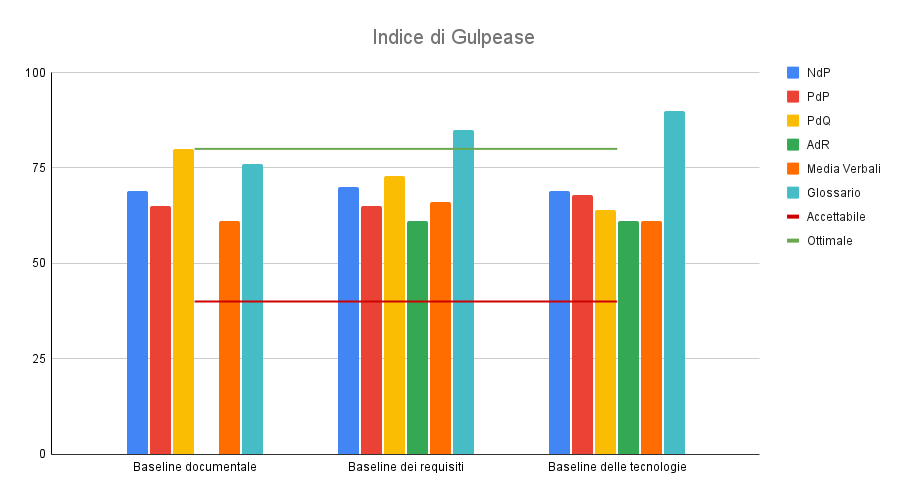
\includegraphics[width=0.8\textwidth, height=0.8\textheight,keepaspectratio]{images/Indice-di-Gulpease.png}
    \caption{Grafico dell'indice di Gulpease dei documenti nei vari periodi.}
\end{figure}    


\subsection{M15VC - Variazione di Costo}
\begin{figure}[H]
    \centering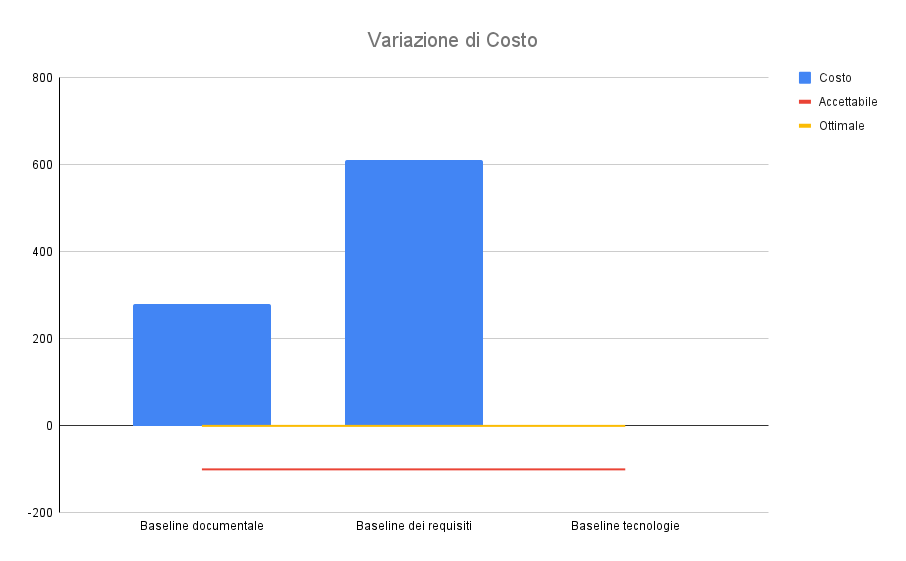
\includegraphics[width=0.8\textwidth, height=0.8\textheight,keepaspectratio]{images/Variazione-di-Costo.png}
    \caption{Grafico che indica come sono variati i costi rispetto a quelli preventivati nei vari periodi.}
\end{figure}    

\subsection{M16VP - Variazione di Piano}
\begin{figure}[H]
    \centering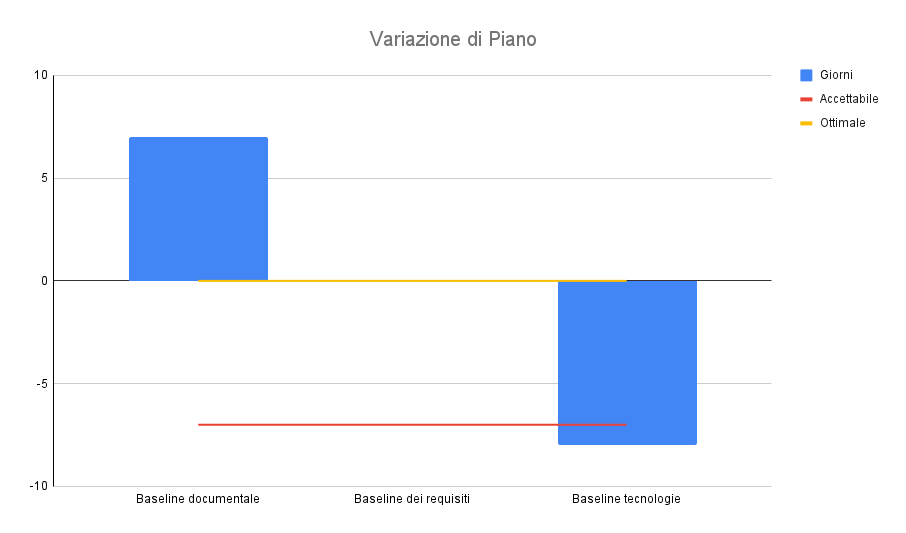
\includegraphics[width=0.8\textwidth, height=0.8\textheight,keepaspectratio]{images/Variazione-di-Piano.png}
    \caption{Grafico che indica come è variata la pianficazione rispetto al preventivo nei vari periodi.}
\end{figure}  
\end{document}